% Chapter Template

\chapter{Results} % Main chapter title

\label{chap:results} 
This chapter will summarize the results of this work. First, the results of simulating the susceptible population (\B{S})
in the region of Hesse will be presented. Then the results of a sensitivity analysis for the variables $\alpha$ and
$q$ will be shown. These are the two variables that are governing the transition from \B{S} to
the Exposed (\B{E}) group ($\alpha$ variable) and transition form \B{E} to the Infected (\B{I}) group ($q$ variable).


%----------------------------------------------------------------------------------------
%	SECTION 1
%----------------------------------------------------------------------------------------

\section{Simulating the susceptible population of Hesse}
\label{sec:sim_res}
\textcolor{red}{Redo image positions :(}

During this work we simulated the susceptible population of Hesse. 26 regions were simulated over a time period of
76, 60 and 50 days respectively. We will show both the absolute and percentage difference between the simulated
and the original data for each time frame.

One challenge of this project was the visualization of the obtained results. Since the number of susceptible
individuals that resign in this group is much greater than the number individuals that transition to the exposed state,
changes in this group are difficult to observe. Because of this we decided against comparing simulated and real world
\B{S} data directly. We instead  calculated and compared the number of individuals that
transitioned from \B{S} to \B{E}. This was done by subtracting the number of susceptible individuals at data point \I{t=x} from
the starting point \I{t=0}. The result is the cumulative change of susceptibles at any given time point, which is equivalent to the 
sum of all exposed individuals at any given time. These results are much easier to visualize, compare and understand.
\textcolor{red}{ADD OPTIMAL VALUES FOR $\alpha$ AND $q$!!}
%-----------------------------------
%	SUBSECTION 1
%-----------------------------------
\subsection{Simulating susceptibles in a 76 day time frame}
We first investigated the accuracy of the model in a time frame of 76 days.
\hyperref[fig:76_sim_expl]{Figure \ref*{fig:76_sim_expl}} shows three graphs. Each of these graphs shows data from the same simulation
process, but different regions. The goal is to show the range of different trends that were present in the data set. Graph A shows
a region where too many infections took place, graph B shows a region where to few transitions took place and finally graph C shows
a region where original and real world transitions are comparable.\newline

\begin{figure}[h]
	\centering
	\begin{subfigure}[b]{0.3\textwidth}
		\centering
		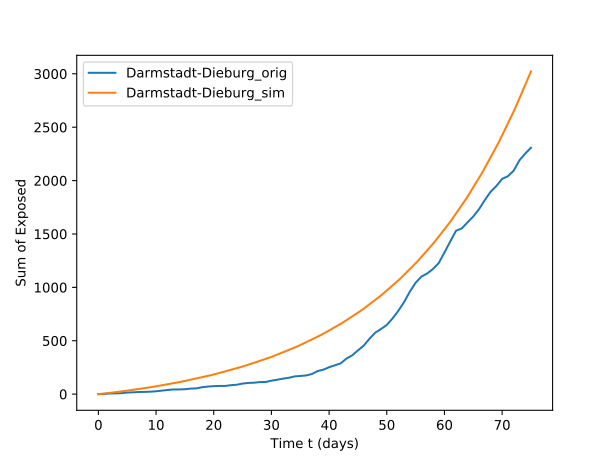
\includegraphics[width=\textwidth]{./figures/76d/24_Darmstadt-Dieburg.png}	
		\caption{}
	\end{subfigure}
	\hfill
	\begin{subfigure}[b]{0.3\textwidth}
		\centering
		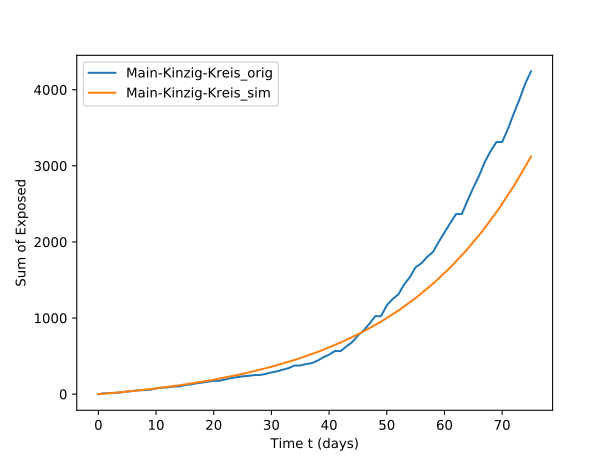
\includegraphics[width=\textwidth]{./figures/76d/13_Main-Kinzig-Kreis.png}	
		\caption{}
	\end{subfigure}
	\hfill
	\begin{subfigure}[b]{0.3\textwidth}
		\centering
		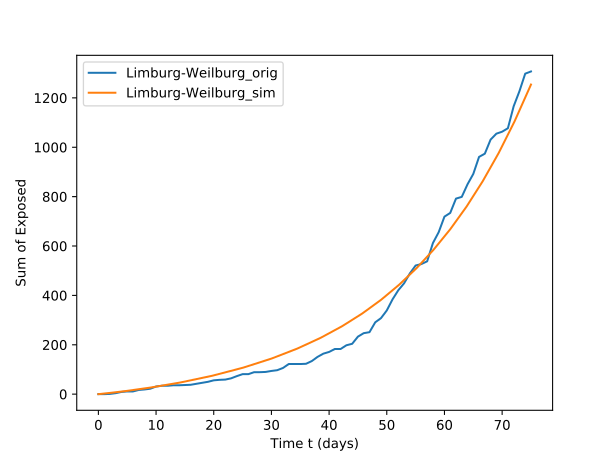
\includegraphics[width=\textwidth]{./figures/76d/10_Limburg-Weilburg.png}	
		\caption{}
	\end{subfigure}
	\caption{Three exemplary results of a simulation of the exposed individuals.
		The original (``orig'') data is drawn in blue and the simulated (``sim'') data is drawn in orange.
		The number of simulated exposed individuals can be greater (image A), smaller 
		(image B) or about the same (image C), as the originally observed number of exposed.
		}
	\label{fig:76_sim_expl}
\end{figure}

In addition, we analyzed the percentage deviation of original and simulated data for each time step in each region. The results
are shown in a box plot in \hyperref[fig:76_sim_box]{figure \ref*{fig:76_sim_box}}. The three regions ``Werra-Meissner-Kreis'',
``Marburg-Biedenkopf'' and ``Limburg-Weilburg'' are listed separately in figure \ref*{fig:76_sim_box}. This was done for scaling reasons,
in order to increase plot readability.\newline

\begin{figure}[h]
	\centering
	\begin{subfigure}[b]{0.4\textwidth}
		\centering
		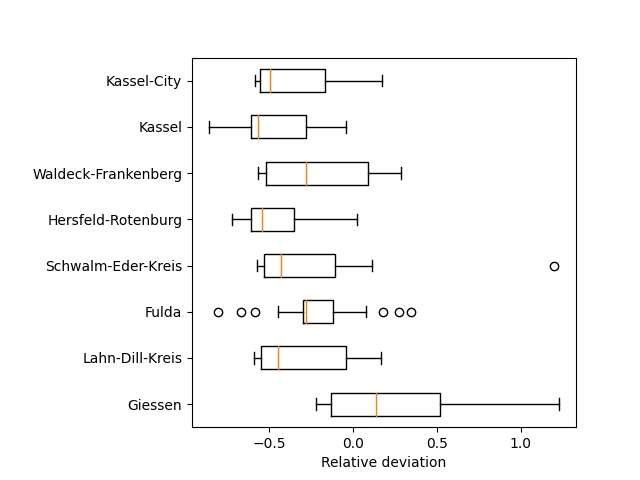
\includegraphics[width=\textwidth]{./figures/76d/deviation_box76_1.png}	
	\end{subfigure}
	\begin{subfigure}[b]{0.4\textwidth}
		\centering
		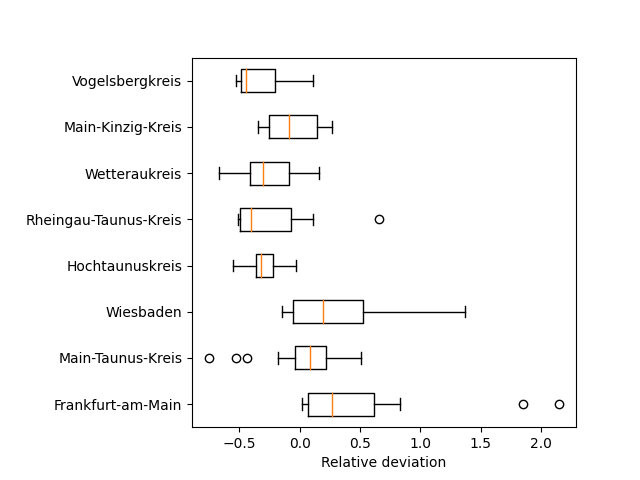
\includegraphics[width=\textwidth]{./figures/76d/deviation_box76_2.png}	
	\end{subfigure}
	\begin{subfigure}[b]{0.4\textwidth}
		\centering
		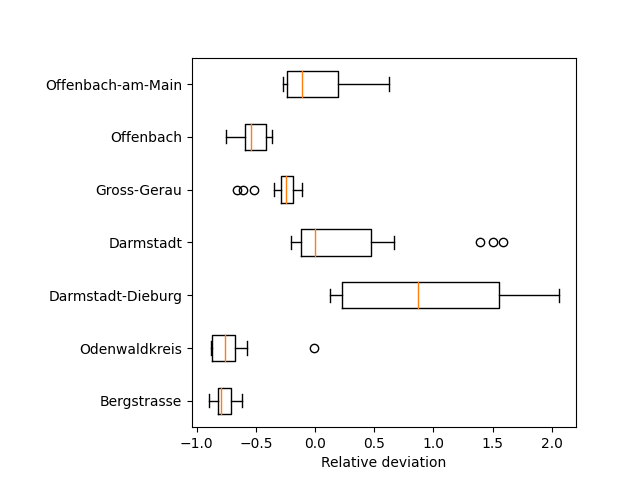
\includegraphics[width=\textwidth]{./figures/76d/deviation_box76_3.png}	
	\end{subfigure}
	\begin{subfigure}[b]{0.4\textwidth}
		\centering
		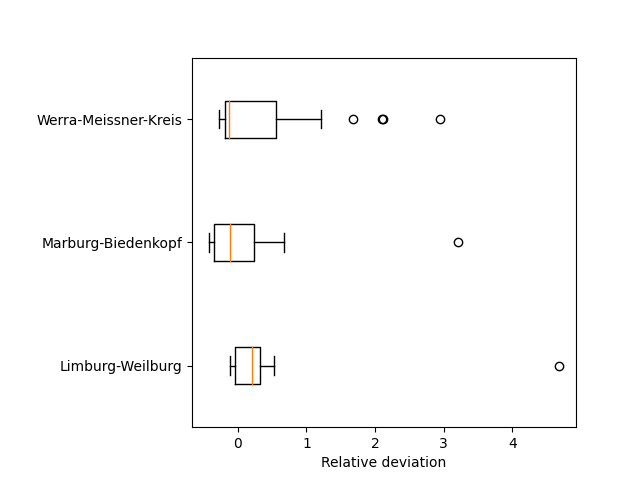
\includegraphics[width=\textwidth]{./figures/76d/deviation_box76_4.png}	
	\end{subfigure}
	\caption{Shown are box plots of the percentage deviation of every simulated region relative to the original data.
		The median deviation ranges between -0.80 and +0.87.}
	\label{fig:76_sim_box}
\end{figure}

Figure \ref*{fig:76_sim_box} shows box plots of the percentage deviation relative to the original data for each time point and region.
For each region all time points were included, unless the real world data had no susceptible transitions at that time. These
time points were ignored in order to avoid divisions by zero.
The numbers are ranging between a median relative deviation of about -0.80 and +0.87. This means, that the model calculated
between 80 percent less or 87 percent more infection events, compared to the original data. Many of the plots are skewed right.
19 of the regions had a median deviation of less than 0 and 7 had a deviation above or at 0.
\hyperref[tab:76d_regions]{Table \ref*{tab:76d_regions}} shows an overview of how many of the 26 regions had an absolute
median deviation below 25, 50 and 75 percent.
\textcolor{red}{add data to Appendix!!!}

\begin{table}[h]
	\centering
	\caption{This table shows the how many of the analyzed regions have an absolute median deviation that is below a given threshold.}
	\begin{tabular}{|l||c|c|c|}
		\hline
		Size of absolute median & $< 0.25$ & $< 0.50$ & $< 0.75$ \\ \hline
		Number of regions & 10 & 20 & 23 \\ \hline
	\end{tabular}
	\label{tab:76d_regions}
\end{table}




%-----------------------------------
%	SUBSECTION 2
%-----------------------------------
\subsection{Simulating susceptibles in a 60 day time frame}
In order to explore how well the model is working with a smaller data set, the same optimization process as in the previous section was
applied to a 60 day data set. Only the first 60 days of the previously chosen time frame were simulated, the other 16 days were
removed. \hyperref[fig:60_sim_expl]{Figure \ref*{fig:60_sim_expl}} shows three exemplary graphs of the simulation results.
For better comparability, the same regions were chosen as in previous section. The results were extrapolated as described previously,
in order to better visualize the trend of the simulation result.\newline

\begin{figure}[h]
	\centering
	\begin{subfigure}[b]{0.3\textwidth}
		\centering
		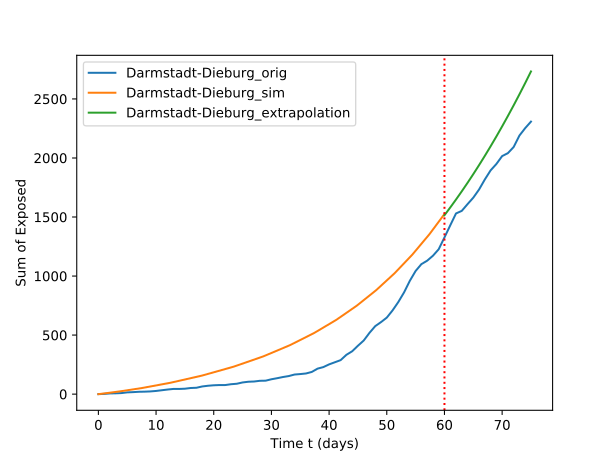
\includegraphics[width=\textwidth]{./figures/60d/24_Darmstadt-Dieburg.png}	
		\caption{}
	\end{subfigure}
	\hfill
	\begin{subfigure}[b]{0.3\textwidth}
		\centering
		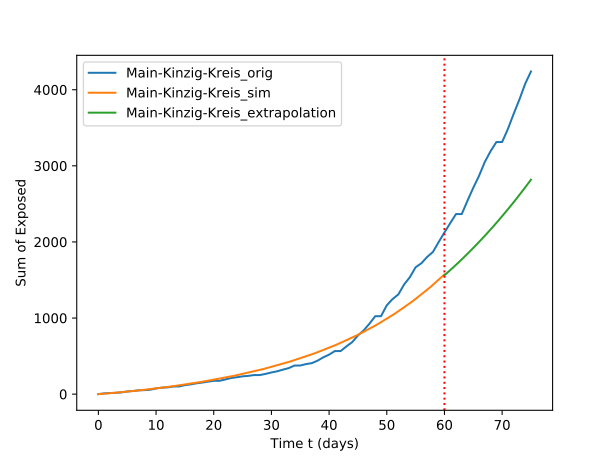
\includegraphics[width=\textwidth]{./figures/60d/13_Main-Kinzig-Kreis.png}	
		\caption{}
	\end{subfigure}
	\hfill
	\begin{subfigure}[b]{0.3\textwidth}
		\centering
		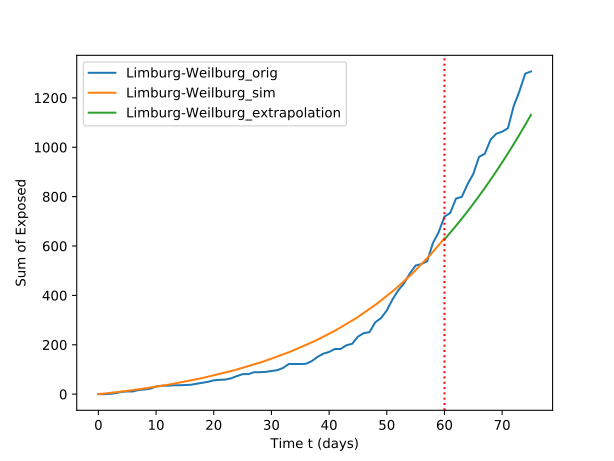
\includegraphics[width=\textwidth]{./figures/60d/10_Limburg-Weilburg.png}	
		\caption{}
	\end{subfigure}
	\caption{Three exemplary results of a simulation of the exposed individuals. The original (``orig'') data is drawn in blue,
		the simulated (``sim'') data is drawn in orange and the extrapolation of the simulated data (``extrapolation'') is
		drawn in green. The vertical red dotted line marks the transition from simulated to extrapolated data.
		}
	\label{fig:60_sim_expl}
\end{figure}

The general trend of the simulations remains similar to the simulations with 76 data points.
In all three regions, the extrapolated data points show a slightly slower increase in number of transitions, compared to the simulations
with 76 days.\newline

Similar to the previous section, we calculated the deviation of each data point for
each region and expressed the results in a set of box plots. The results are shown in \hyperref[fig:60_sim_box]{figure \ref*{fig:60_sim_box}}. Only data points
that were actually simulated were included into this analysis. Extrapolated data points were excluded.\newline

\begin{figure}[h]
	\centering
	\begin{subfigure}[b]{0.4\textwidth}
		\centering
		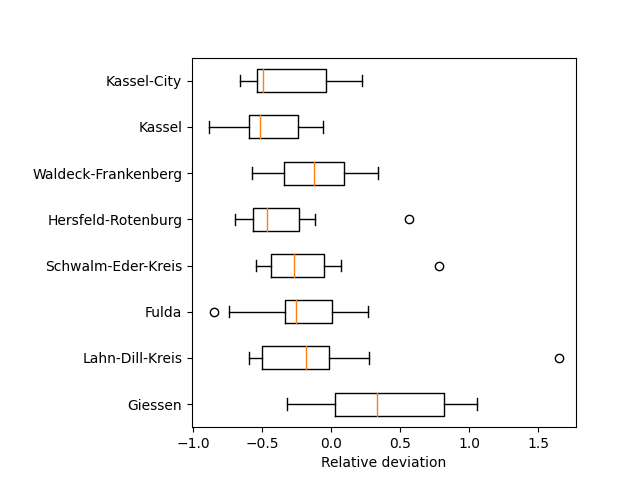
\includegraphics[width=\textwidth]{./figures/60d/deviation_box60_1.png}	
	\end{subfigure}
	\begin{subfigure}[b]{0.4\textwidth}
		\centering
		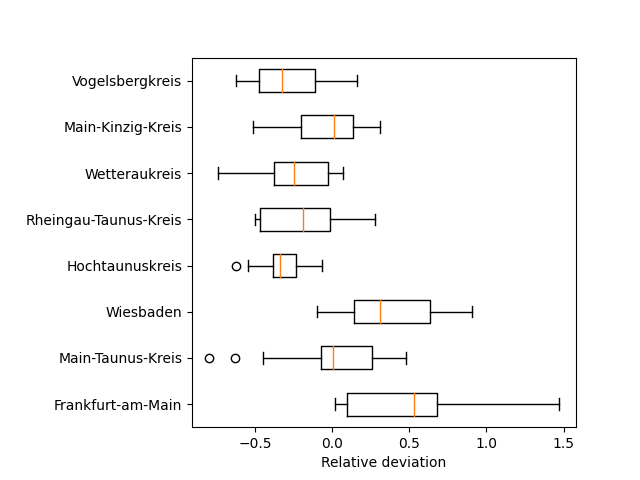
\includegraphics[width=\textwidth]{./figures/60d/deviation_box60_2.png}	
	\end{subfigure}
	\begin{subfigure}[b]{0.4\textwidth}
		\centering
		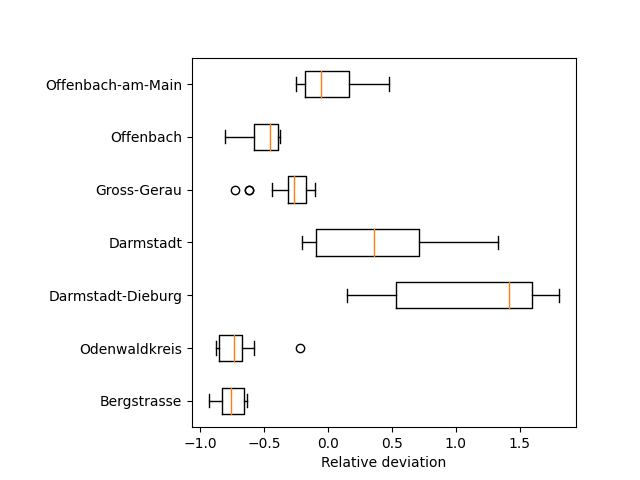
\includegraphics[width=\textwidth]{./figures/60d/deviation_box60_3.png}	
	\end{subfigure}
	\begin{subfigure}[b]{0.4\textwidth}
		\centering
		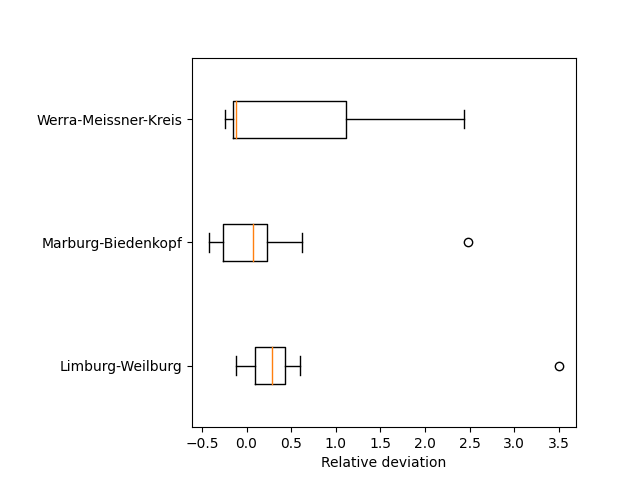
\includegraphics[width=\textwidth]{./figures/60d/deviation_box60_4.png}	
	\end{subfigure}
	\caption{Shown are box plots of the percentage deviation relative to the real world data. 
		Only 60 of 76 data points were. The median of all simulated regions ranges between -0.76 and 1.42.
		}
	\label{fig:60_sim_box}
\end{figure}

The deviation results of the 60 data point simulations are largely comparable to the 76 data point deviation results.
The minimum median deviation is slightly lower compared to the previous simulation at -76, while the maximum deviation is higher at 142 percent. 
Again many of the plots are skewed right, however a number of plots is also skewed left. 17 of the regions had a median deviation of less than
0, while 9 regions had a deviation of 0 or higher. \hyperref[tab:60d_regions]{Table \ref*{tab:60d_regions}} shows how many of the 26 regions had
absolute median deviation below 25, 50 and 75 percent.

\begin{table}[h]
	\centering
	\caption{This table shows the how many of the analyzed regions have an absolute median deviation that is below a given threshold.}
	\begin{tabular}{|l||c|c|c|}
		\hline
		Size of absolute median & $< 0.25$ & $< 0.50$ & $< 0.75$ \\ \hline
		Number of regions & 9 & 21 & 24 \\ \hline
	\end{tabular}
	\label{tab:60d_regions}
\end{table}

%-----------------------------------
%	SUBSECTION 3
%-----------------------------------
\subsection{Simulating susceptibles in a 50 day time frame}
The last simulation was performed with 50 data points. As described in the previous section with 60 data points, simulations and
optimization steps were done on a truncated data set, where the last 26 of the total 76 data points were removed.
\hyperref[fig:50_sim_expl]{Figure \ref*{fig:50_sim_expl}} shows three exemplary graphs of this
experiment. The same regions were chosen as for the 76 data point experiment. 

\begin{figure}[h]
	\centering
	\begin{subfigure}[b]{0.3\textwidth}
		\centering
		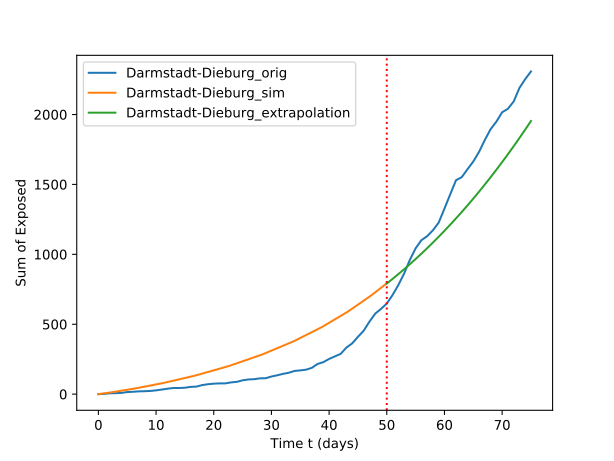
\includegraphics[width=\textwidth]{./figures/50d/24_Darmstadt-Dieburg.png}	
		\caption{}
	\end{subfigure}
	\hfill
	\begin{subfigure}[b]{0.3\textwidth}
		\centering
		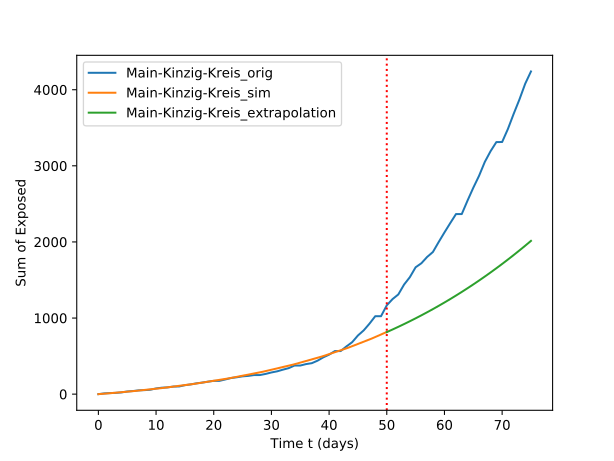
\includegraphics[width=\textwidth]{./figures/50d/13_Main-Kinzig-Kreis.png}	
		\caption{}
	\end{subfigure}
	\hfill
	\begin{subfigure}[b]{0.3\textwidth}
		\centering
		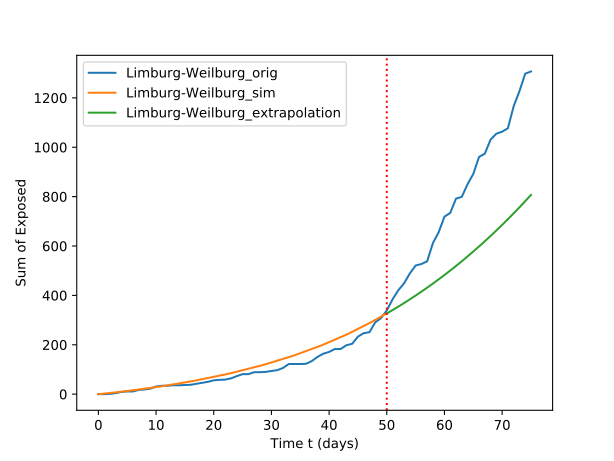
\includegraphics[width=\textwidth]{./figures/50d/10_Limburg-Weilburg.png}	
		\caption{}
	\end{subfigure}
	\caption{Add caption
		}
	\label{fig:50_sim_expl}
\end{figure}
All three regions show a stronger trend towards a negative deviation compared to the results of the previous two experiments.
While the simulated regions looks similar to the real world data, the extrapolation shows a strong deviation towards too little susceptible
transitions.\newline

Analogous to the 60 data point data set, we also performed the deviation analysis on the 50 data point data set. The results of this
analysis are shown in \hyperref[fig:50_sim_box]{Figure \ref*{fig:50_sim_box}}.\newline

\begin{figure}[h]
	\centering
	\begin{subfigure}[b]{0.4\textwidth}
		\centering
		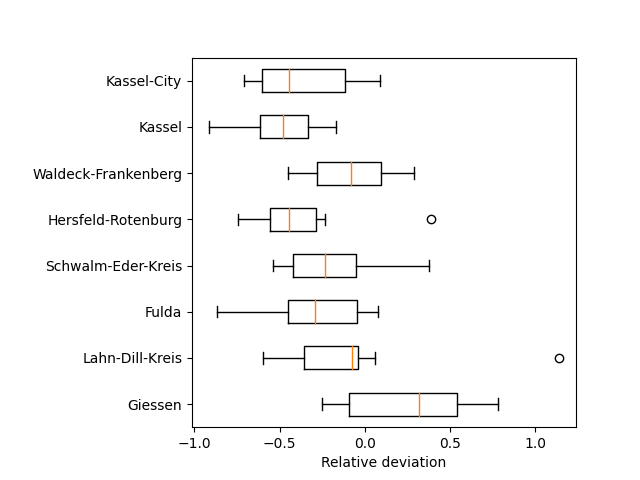
\includegraphics[width=\textwidth]{./figures/50d/deviation_box50_1.png}	
	\end{subfigure}
	\begin{subfigure}[b]{0.4\textwidth}
		\centering
		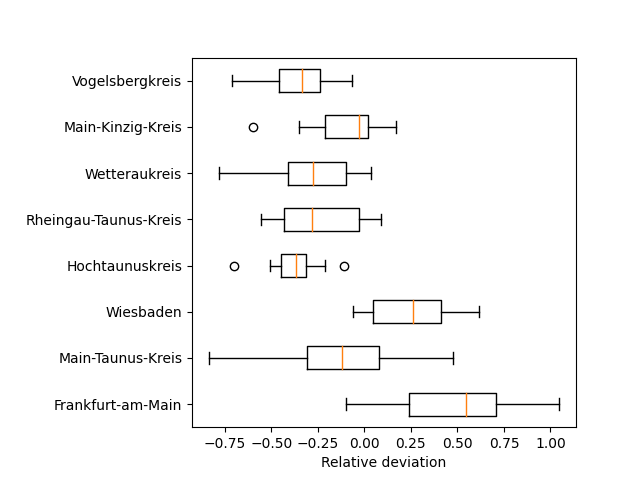
\includegraphics[width=\textwidth]{./figures/50d/deviation_box50_2.png}	
	\end{subfigure}
	\begin{subfigure}[b]{0.4\textwidth}
		\centering
		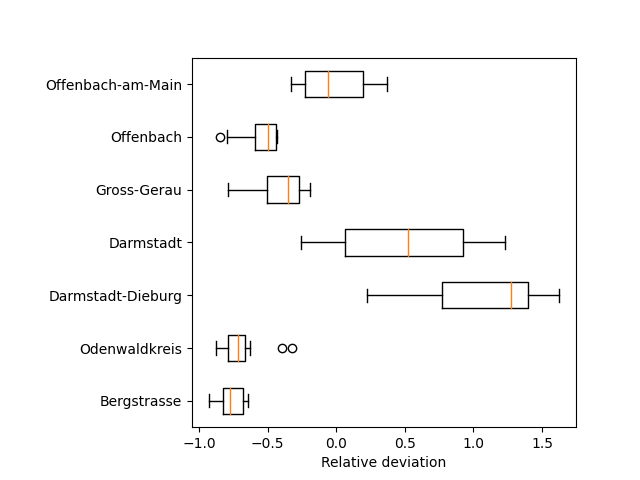
\includegraphics[width=\textwidth]{./figures/50d/deviation_box50_3.png}	
	\end{subfigure}
	\begin{subfigure}[b]{0.4\textwidth}
		\centering
		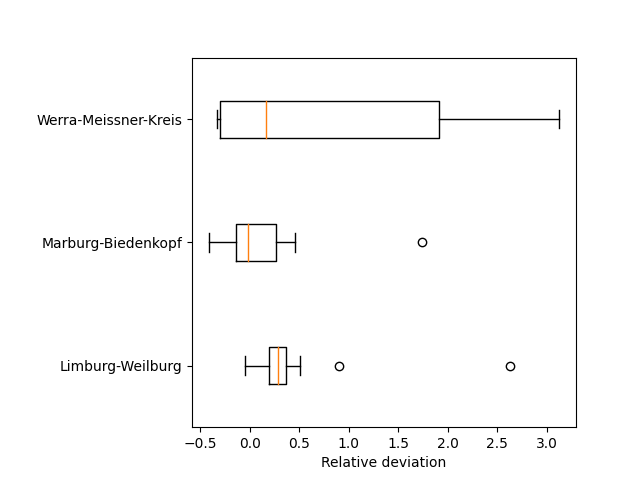
\includegraphics[width=\textwidth]{./figures/50d/deviation_box50_4.png}	
	\end{subfigure}
	\caption{Shown are box plots of the percentage deviation relative to the real world data for every region. Only 50
		of the 76 data points were simulated. The median deviation of all regions ranges between -0.77 and 1.27.		}
	\label{fig:50_sim_box}
\end{figure}

The 50 data point simulations show similar results to the previous two experiments. The median deviation of all regions
ranges between -77 and +127 percent. 19 of the simulated regions had a median deviation below 0 and 7 regions had a
median deviation of 0 or higher. Many of the plots appear to be skewed either left or right.
\hyperref[tab:50d_regions]{Table \ref*{tab:50d_regions}} shows how many regions had a deviation of less than 25, 50 and 75
percent respectively.\newline

\begin{table}[h]
	\centering
	\caption{This table shows the how many of the analyzed regions have an absolute median deviation that is below a given threshold.}
	\begin{tabular}{|l||c|c|c|}
		\hline
		Size of absolute median & $< 0.25$ & $< 0.50$ & $< 0.75$ \\ \hline
		Number of regions & 8 & 21 & 24 \\ \hline
	\end{tabular}
	\label{tab:50d_regions}
\end{table}

%----------------------------------------------------------------------------------------
%	SECTION 2
%----------------------------------------------------------------------------------------

\section{Influence of individual regions on the loss function}
In order to better understand the influence of individual regions on the model itself, we manually calculated the total
loss, the individual loss for each region and the percentage loss of each region relative to the total loss.
\hyperref[tab:perc_region_loss]{Table \ref*{tab:perc_region_loss}} shows the results of these calculations. The table
is sorted descending from highest to lowest percentage loss contribution.
\textcolor{red}{add table with total information to Appendix}

\begin{table}[h]
	\caption{the caption}
	\begin{tabular}{|l|x{2cm}|x{2cm}|x{2cm}|}
	%\begin{tabular}{|l|c|c|c|}
		\hline
		\B{region} & \B{percentage loss} & \B{percentage population} & \B{median deviation} \\ \hline \hline
		Offenbach & 27.70 & 5.67 & -0.54 \\ \hline
		Bergstrasse & 14.41 & 4.31 & -0.79 \\ \hline
		Frankfurt-am-Main & 13.10 & 12.14 & 0.21 \\ \hline
		Lahn-Dill-Kreis & 6.29 & 4.03 & -0.25 \\ \hline
		Main-Kinzig-Kreis & 5.17 & 6.70 & -0.07 \\ \hline
		Marburg-Biedenkopf & 4.70 & 3.91 & -0.06 \\ \hline
		Kassel-City & 3.90 & 3.19 & -0.49 \\ \hline
		Wetteraukreis & 3.35 & 4.93 & -0.27 \\ \hline
		Gross-Gerau & 2.90 & 4.38 & -0.23 \\ \hline
		Rheingau-Taunus-Kreis & 2.89 & 2.98 & -0.36 \\ \hline
		Kassel & 2.58 & 3.77 & -0.55 \\ \hline
		Hochtaunuskreis & 2.33 & 3.77 & -0.32 \\ \hline
		Darmstadt-Dieburg & 2.00 & 4.73 & 0.74 \\ \hline
		Odenwaldkreis & 1.93 & 1.54 & -0.75 \\ \hline
		Offenbach-am-Main & 1.23 & 2.08 & -0.09 \\ \hline
		Schwalm-Eder-Kreis & 1.03 & 2.86 & -0.34 \\ \hline
		Waldeck-Frankenberg & 0.99 & 2.49 & -0.17 \\ \hline
		Giessen & 0.84 & 4.32 & 0.10 \\ \hline
		Wiesbaden & 0.80 & 4.43 & 0.17 \\ \hline
		Fulda & 0.74 & 3.54 & -0.28 \\ \hline
		Hersfeld-Rotenburg & 0.41 & 1.91 & -0.48 \\ \hline
		Main-Taunus-Kreis & 0.25 & 3.80 & 0.07 \\ \hline
		Darmstadt & 0.18 & 2.53 & 0.00 \\ \hline
		Vogelsbergkreis & 0.17 & 1.68 & -0.37 \\ \hline
		Limburg-Weilburg & 0.08 & 2.74 & 0.11 \\ \hline
		Werra-Meissner-Kreis & 0.03 & 1.59 & -0.11 \\ \hline
	\end{tabular}
	\label{tab:perc_region_loss}
\end{table}

The results show, that the main contribution of the loss function is done by a minority of regions. The top three contributors
account for 55.21 percent of the entire loss, while only making up about 22.12 percent of the total population. The top seven
contributors make up about 75.27 percent, while making up about 39.95 percent of the population. A notable find is, that the
top two regions, ``Offenbach'' and ``Bergstrasse'', both display a negative deviation, while the third most influential region
``Frankfurt-am-Main'' has a positive deviation. Frankfurt also has a lower overall contribution to the loss, than the other
two regions, even though it has a higher share of the total population then the other two regions combined.

%----------------------------------------------------------------------------------------
%	SECTION 3
%----------------------------------------------------------------------------------------

\section{Sensitivity analysis of $\alpha$ and $q$}
\textcolor{red}{add more angles to the images}
In order to further investigate the features of the model, we analyzed the sensitivity of the loss function relative to
the variables $\alpha$ and $q$. We only chose those two variables, since the loss function was only calculated based
on the difference between the simulated and the original susceptible population. Since this group only depends on those
two variables in our model, changes in the other variables could not influence the loss and were therefore not investigated.
For this experiment, the 4000 simulations of the model with all 76 original data points were performed and the variables
$\alpha$ and $q$ were chosen randomly, within a set constraint. The upper and lower bounds were set to 0.05 and 0.35 for 
$\alpha$ and 5.5 and 8.0 for $q$ respectively. The results of these simulations were gathered and used to plot a map
of the variable landscape of the loss of the susceptible group.
\hyperref[fig:sensitivity_zoom0]{Figure \ref*{fig:sensitivity_zoom0}} shows the total result of all simulations over the
chosen bounds.

\begin{figure}[h]
	\centering
	\begin{subfigure}[b]{0.4\textwidth}
		\centering
		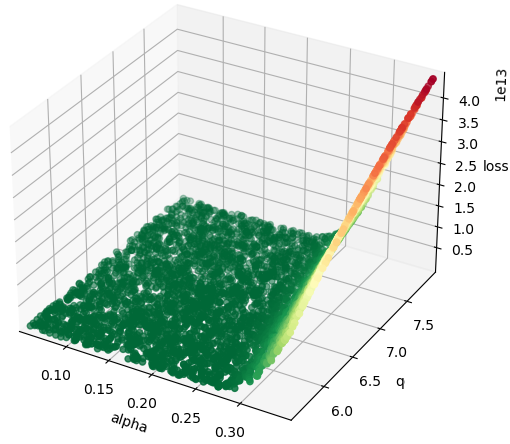
\includegraphics[width=\textwidth]{./figures/sensitivity/sensitivity_zoom0_0_2.png}	
		\caption{}
	\end{subfigure}
	\begin{subfigure}[b]{0.4\textwidth}
		\centering
		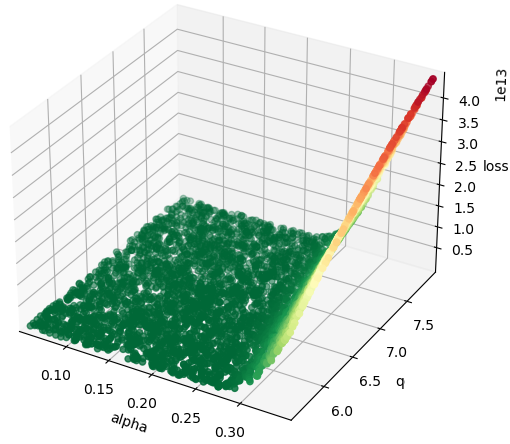
\includegraphics[width=\textwidth]{./figures/sensitivity/sensitivity_zoom0_0_2.png}	
		\caption{}
	\end{subfigure}
	\caption{Visualization of the variable sensitivity of the susceptible group. The variables $\alpha$ and $q$ were plotted
		against the loss of the susceptible group. Images (A) and (B) show the plot from different angles in order
		to increase readability. In the model the susceptible group shows sensitivity to changes of both $\alpha$ and
		$q$. However, the sensitivity to $q$ seems to be dependent on $\alpha$.
		}
	\label{fig:sensitivity_zoom0}
\end{figure}

\textcolor{red}{add result values to figure explanation}
Figure \ref*{fig:sensitivity_zoom0} shows that low values for $\alpha$ lead to a decreased sensitivity of the loss function
for $q$. Only after an $\alpha$ value of about 0.25 is reached, does the loss start to react to changes in $q$. After this point
however, the loss function quickly increases. This phenomenon can be seen both, if $q$ is increased and if $q$ is not increased
in the simulation. But a bigger $q$ value causes the loss to increase more quickly compared to a simulation with a small loss.



The simulations were further investigated by plotting only part of the experimental data.
The first row of \hyperref[fig:sensitivity_zoom0]{Figure \ref*{fig:sensitivity_zoom0}} shows all data points with $\alpha$ values between 0.15
and 0.25, $q$ values between 5.5 and 8.0 and a maximum loss of $10^{10}$. The loss on this image was capped in order to reduce
the scale of the loss and thereby increase readability. This lead 957 of 4000 data points being plotted. The images in the
second row show the same graph (\textcolor{red}{?}), with the same bonds for $\alpha$ and $q$, but with a maximum loss capped
at $2.7*10^{9}$. This gives an even closer look at the range of optimal/close-to-optimal values for $\alpha$ and $q$.

\begin{figure}[h]
	\centering
	\begin{subfigure}[b]{0.4\textwidth}
		\centering
		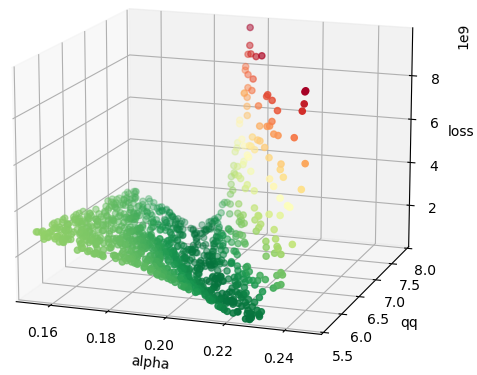
\includegraphics[width=\textwidth]{./figures/sensitivity/sensitivity_zoom1_0_2.png}	
	\end{subfigure}
	\begin{subfigure}[b]{0.4\textwidth}
		\centering
		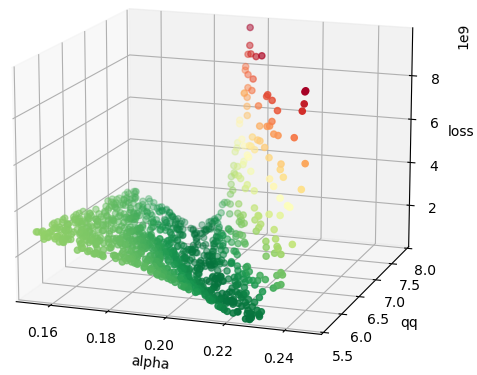
\includegraphics[width=\textwidth]{./figures/sensitivity/sensitivity_zoom1_0_2.png}	
	\end{subfigure}
	\begin{subfigure}[b]{0.4\textwidth}
		\centering
		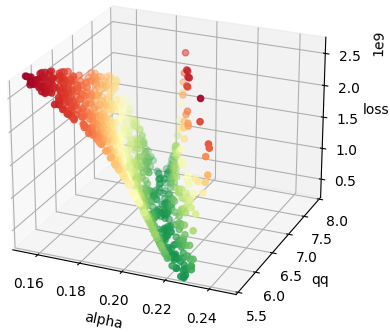
\includegraphics[width=\textwidth]{./figures/sensitivity/sensitivity_zoom2_0_2.png}	
	\end{subfigure}
	\begin{subfigure}[b]{0.4\textwidth}
		\centering
		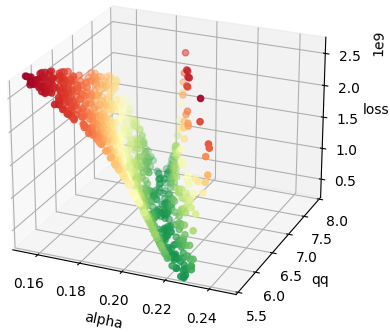
\includegraphics[width=\textwidth]{./figures/sensitivity/sensitivity_zoom2_0_2.png}	
	\end{subfigure}
	\caption{Visualization of the variable sensitivity of the susceptible group. The variables $\alpha$ and $q$ were
		capped to 0.15 and 0.25 and 5.5 and 8.0 respectively and then plotted against the result of the loss function.
		The loss was capped at $10^{10}$ and $2.7*10^{9}$ for the first and the second row respectively, in order to
		reduce the scale of the loss and make the image more readable. The image shows that there seems to be a set of
		optimal value combinations of $\alpha$ and $q$, where the loss is minimized. Given the diagonal nature of this
		``optimal cavity'' there seem to be an equilibrium between the two values.
		\textcolor{red}{check for better wording} %note
		}
	\label{fig:sensitivity_zoom1}
\end{figure}

Figure \ref*{fig:sensitivity_zoom1} shows the existence of a ``valley'' with minimized loss. It can be seen that there are 
sets of values of $\alpha$ and $q$, where the loss appears to be minimized. The optimal values found by the model for $\alpha$
and $q$ are also withing this region (\textcolor{red}{more info}). The optimized area seems to have a diagonal structure,
indicating an optimal relation between $\alpha$ and $q$.

